\documentclass{article}
\usepackage[margin=0.75in]{geometry}
\usepackage{tikz}
\usetikzlibrary{positioning,arrows.meta,calc,fit,backgrounds}
\usepackage{tcolorbox}
\usepackage{xcolor}
\usepackage{skak}

\newcommand{\benchmark}{ChessChain}

\begin{document}

\begin{figure}[t]
    \centering

    % Chess problem - Version 5: Linear left-to-right flow (like chemistry v2)
    \begin{tcolorbox}[
        title=\textbf{Chess: Minimax Search} \hfill {\small\colorbox{orange!20}{Easy} \quad 6 orderings},
        colframe=orange!70!black,
        colback=orange!3,
        boxrule=0.8pt,
        width=\textwidth
    ]
    \small

    \textbf{Dependency graph:}
    \begin{center}
    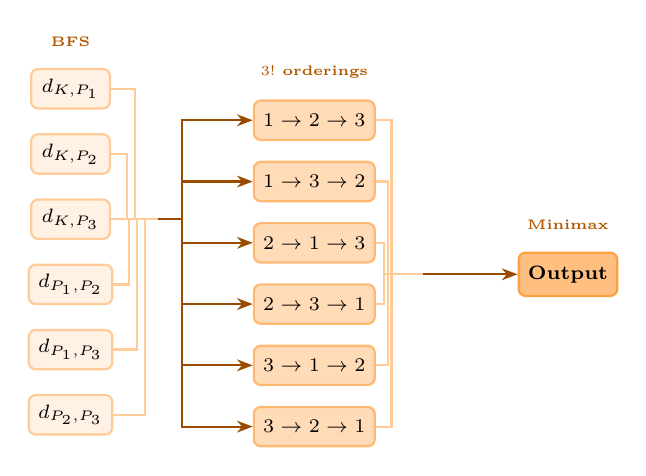
\begin{tikzpicture}[
        node distance=0.6cm and 1.0cm,
        every node/.style={font=\scriptsize},
        bfs/.style={draw, rounded corners=2.5pt, fill=orange!10, minimum width=1.0cm, minimum height=0.5cm, thick, draw=orange!40},
        ordnode/.style={draw, rounded corners=2.5pt, fill=orange!28, minimum width=1.1cm, minimum height=0.5cm, thick, draw=orange!55},
        outputnode/.style={draw, rounded corners=2.5pt, fill=orange!50, minimum width=1.0cm, minimum height=0.55cm, thick, draw=orange!75, font=\scriptsize\bfseries},
        arrow/.style={-{Stealth[length=2mm]}, thick, orange!60!black}
    ]
        % Column 1: BFS distances (stacked vertically)
        \node[bfs] (b1) {$d_{K,P_1}$};
        \node[bfs, below=0.3cm of b1] (b2) {$d_{K,P_2}$};
        \node[bfs, below=0.3cm of b2] (b3) {$d_{K,P_3}$};
        \node[bfs, below=0.3cm of b3] (b4) {$d_{P_1,P_2}$};
        \node[bfs, below=0.3cm of b4] (b5) {$d_{P_1,P_3}$};
        \node[bfs, below=0.3cm of b5] (b6) {$d_{P_2,P_3}$};

        % Column 2: Orderings (stacked vertically, offset to center)
        \node[ordnode, right=1.8cm of b1, yshift=-0.4cm] (o1) {$1 \to 2 \to 3$};
        \node[ordnode, below=0.25cm of o1] (o2) {$1 \to 3 \to 2$};
        \node[ordnode, below=0.25cm of o2] (o3) {$2 \to 1 \to 3$};
        \node[ordnode, below=0.25cm of o3] (o4) {$2 \to 3 \to 1$};
        \node[ordnode, below=0.25cm of o4] (o5) {$3 \to 1 \to 2$};
        \node[ordnode, below=0.25cm of o5] (o6) {$3 \to 2 \to 1$};

        % Column 3: Output
        \node[outputnode, right=1.8cm of o3, yshift=-0.4cm] (out) {Output};

        % Arrows from BFS to orderings (use a gathering point)
        \coordinate (gather1) at ($(b3.east) + (0.6cm, 0)$);

        % Draw arrows from BFS nodes to gather point
        \draw[orange!40, thick] (b1.east) -- ++(0.3cm,0) |- (gather1);
        \draw[orange!40, thick] (b2.east) -- ++(0.2cm,0) |- (gather1);
        \draw[orange!40, thick] (b3.east) -- (gather1);
        \draw[orange!40, thick] (b4.east) -- ++(0.2cm,0) |- (gather1);
        \draw[orange!40, thick] (b5.east) -- ++(0.3cm,0) |- (gather1);
        \draw[orange!40, thick] (b6.east) -- ++(0.4cm,0) |- (gather1);

        % Draw arrows from gather point to orderings
        \draw[arrow] (gather1) -- ++(0.3cm,0) |- (o1.west);
        \draw[arrow] (gather1) -- ++(0.3cm,0) |- (o2.west);
        \draw[arrow] (gather1) -- ++(0.3cm,0) |- (o3.west);
        \draw[arrow] (gather1) -- ++(0.3cm,0) |- (o4.west);
        \draw[arrow] (gather1) -- ++(0.3cm,0) |- (o5.west);
        \draw[arrow] (gather1) -- ++(0.3cm,0) |- (o6.west);

        % Arrows from orderings to output (use a gathering point)
        \coordinate (gather2) at ($(o3.east) + (0.6cm, -0.4cm)$);

        \draw[orange!40, thick] (o1.east) -- ++(0.2cm,0) |- (gather2);
        \draw[orange!40, thick] (o2.east) -- ++(0.15cm,0) |- (gather2);
        \draw[orange!40, thick] (o3.east) -- ++(0.1cm,0) |- (gather2);
        \draw[orange!40, thick] (o4.east) -- ++(0.1cm,0) |- (gather2);
        \draw[orange!40, thick] (o5.east) -- ++(0.15cm,0) |- (gather2);
        \draw[orange!40, thick] (o6.east) -- ++(0.2cm,0) |- (gather2);

        \draw[arrow] (gather2) -- (out.west);

        % Labels
        \node[font=\tiny\bfseries, orange!70!black, anchor=south] at ([yshift=0.15cm]b1.north) {BFS};
        \node[font=\tiny\bfseries, orange!70!black, anchor=south] at ([yshift=0.15cm]o1.north) {$3!$ orderings};
        \node[font=\tiny\bfseries, orange!70!black, anchor=south] at ([yshift=0.15cm]out.north) {Minimax};

    \end{tikzpicture}
    \end{center}

    \vspace{-0.1cm}
    \begin{tabular}{@{}p{0.48\textwidth}p{0.48\textwidth}@{}}
    \textit{Step 1:} BFS computes all 6 pairwise knight distances between $K$, $P_1$, $P_2$, $P_3$. &
    \textit{Step 2:} Each ordering sums its path distances; minimax finds optimal play (Alice MAX, Bob MIN). \\
    \end{tabular}

    \vspace{0.15cm}
    \hfill \textbf{Answer:} [Redacted]
    \end{tcolorbox}

    \caption{\textbf{Chess dependency graph:} Left-to-right flow showing \colorbox{orange!10}{BFS distances} feeding all \colorbox{orange!28}{$3!$ orderings}, which are evaluated via \colorbox{orange!50}{minimax}.}
\end{figure}

\end{document}
